%=== CHAPTER TWO (2) ===

\chapter{MDA}

This chapter discusses the mechanics, dynamics and aesthetics of the game. We refer agent tank to the tank that is stationary in the center of map and it is fully autonomous. To achieve the intelligence for autonomous control, it trains a NN model using reinforcement learning. Further details will be discussed in Chapter 3. 
\FloatBarrier

\label{sec:MDA}

\section{Mechanics}

\subsection{Agent Tank}
The agent tank's actions are controlled autonomously via function approximator (i.e. deep neural network) trained using UnityML's reinforcement learning framework. This framework is implemented using Tensorflow\cite{goldsborough2016tour} and communicates and with unity editor via an API implemented using python. 


The agent has the action to shoot, and rotate about the same position. It does not have the ability to move. The agent tank uses Unity's \textit{RayPerceptionSensor} \cite{majumder2021understanding} module to differentiate the enemy tanks from friendly tanks as they are tagged differently.

\subsection{Enemy AI}
\begin{figure*}[t]
\centering
\begin{multicols}{2}
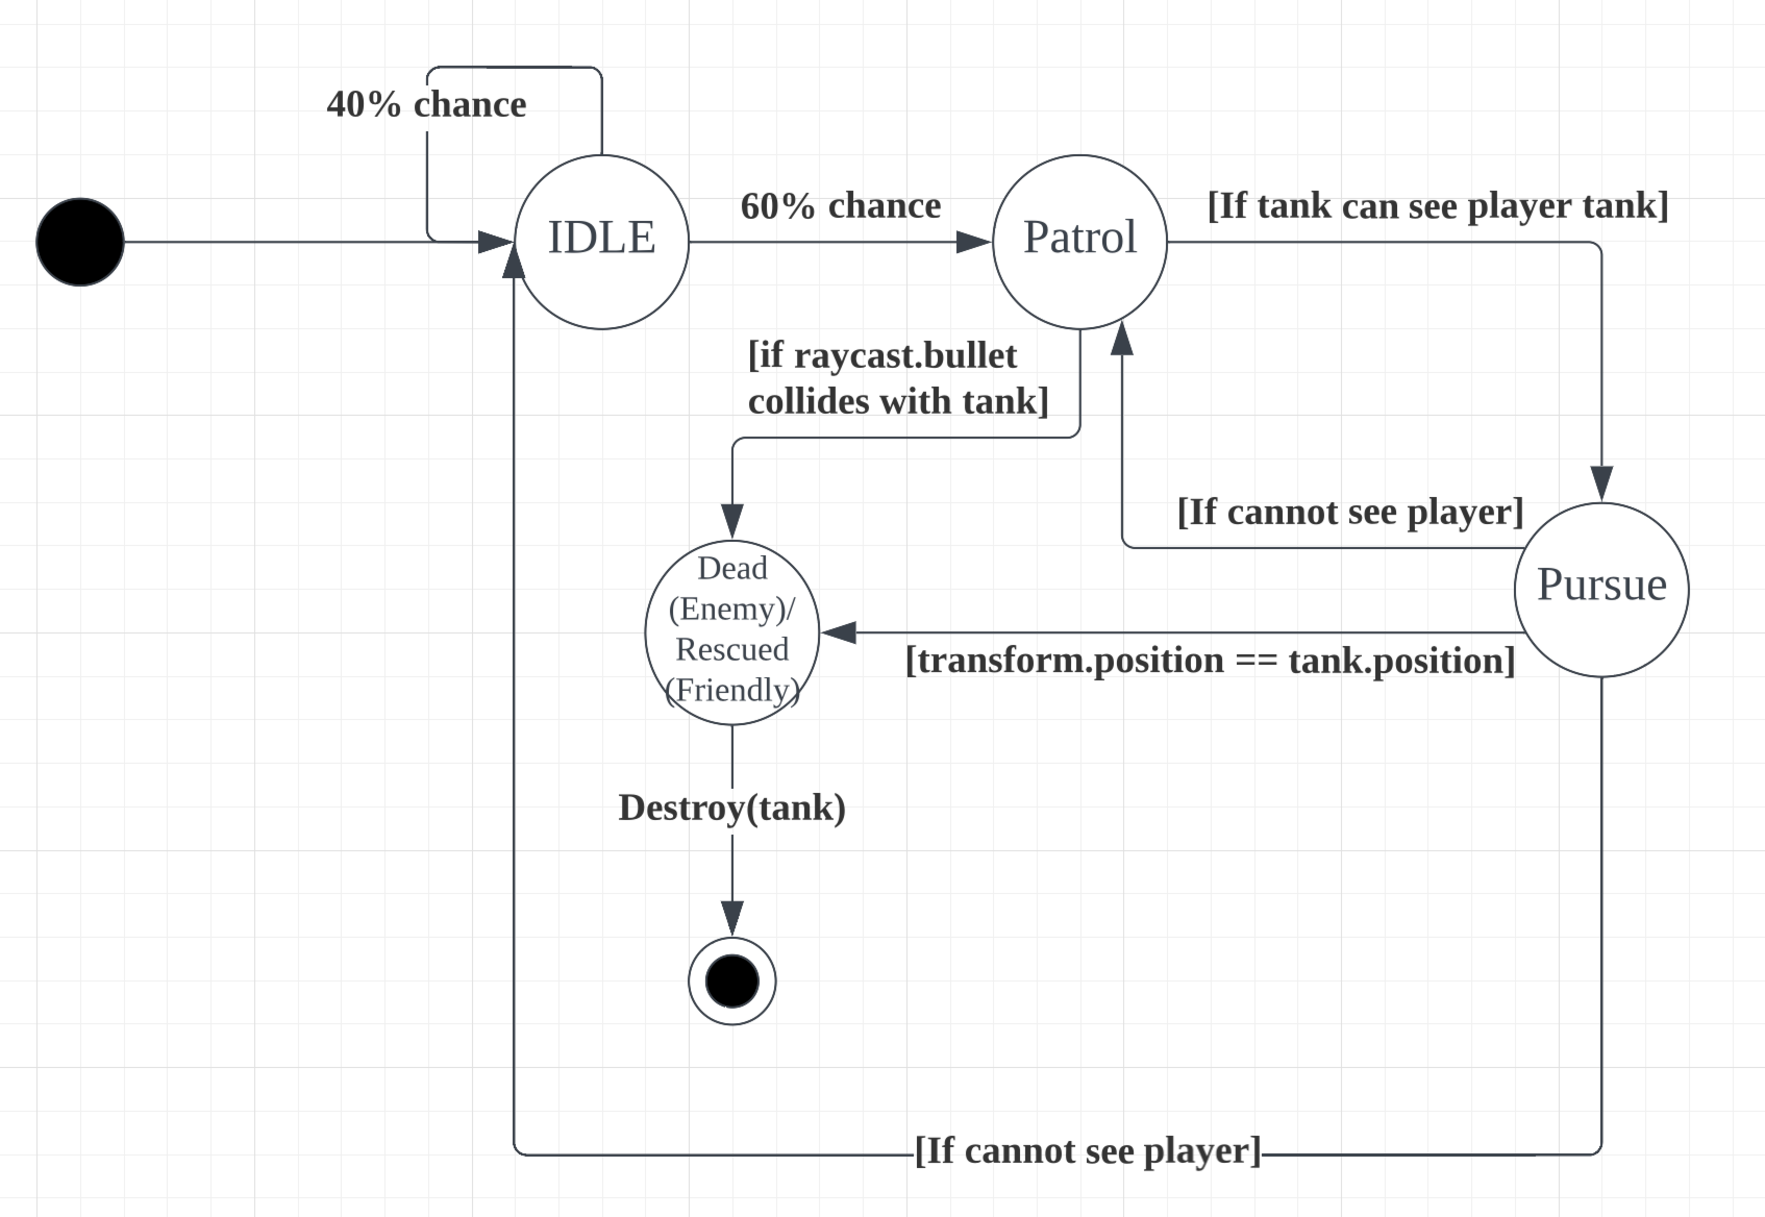
\includegraphics[width=0.99\columnwidth]{Chapter2/Enemy_AI.pdf}
\caption{Finite state machine for enemy and friendly tanks}
\label{fig:FSM_enemy}

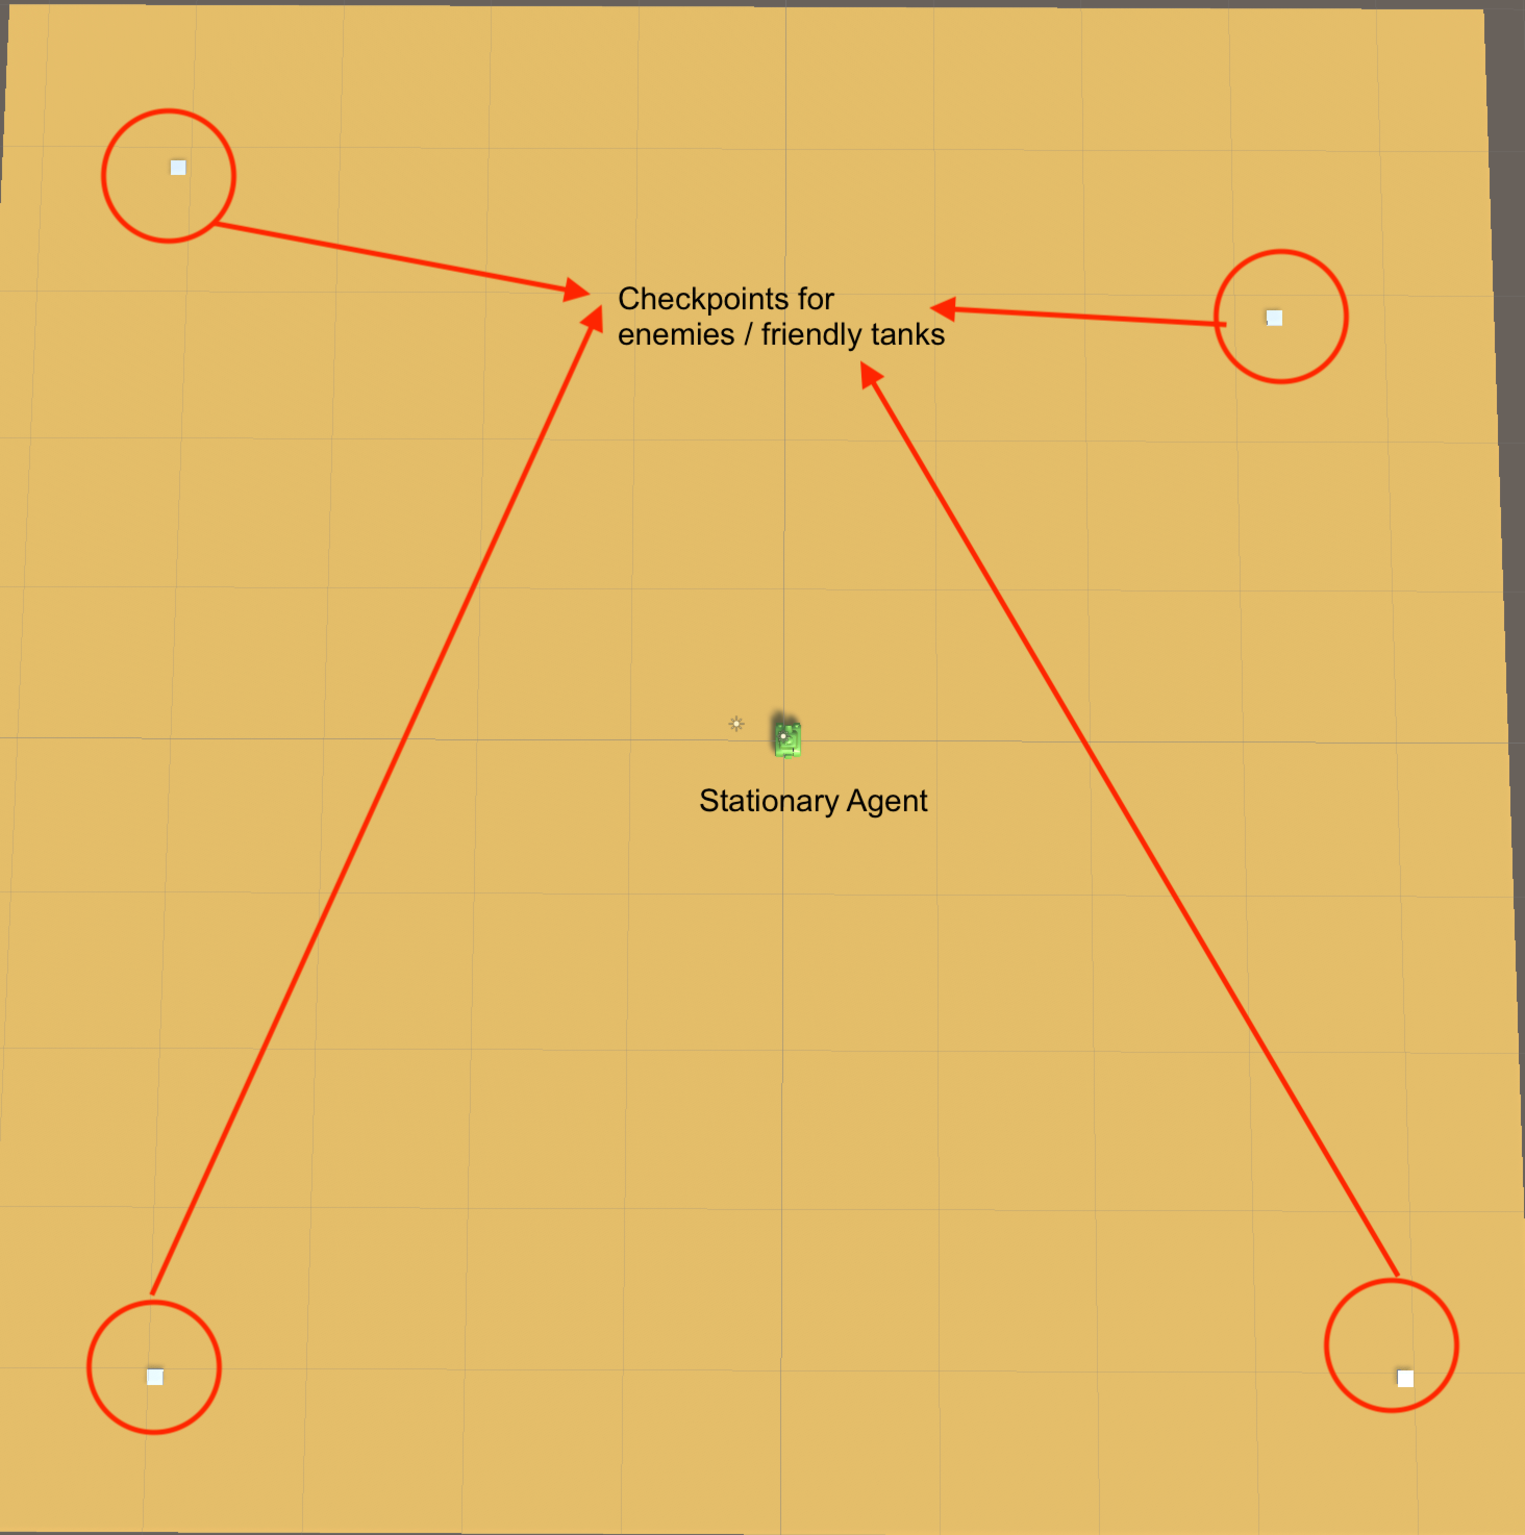
\includegraphics[width=0.99\columnwidth, height=0.7\columnwidth]{Chapter2/Map.pdf}
\caption{Finite state machine for enemy and friendly tanks}
\label{fig:Map}

\end{multicols}
\end{figure*}

The enemy and friendly follows a finite state machine (FSM) as depicted in Figure. \ref{fig:FSM_enemy}. Although both tanks follow the same FSM, the agent differentiates them using Unity's tag system and allocate rewards accordingly.

We used "checkpoints" to guide the enemy tanks in the area where they should patrol. These checkpoints are effectively way-points that are placed in the four corners of the map. This way, the enemy tanks will visit these way-points in an orderly manner, creating the illusion that they are patrolling. Similar to Assignment 1 the \textit{NavMeshAgent} from Unity3D was utilized for enemy and friendly tank’s ability to move around the map. 

\section{Dynamics}

Enemy and Friendly tanks are spawned randomly around the map such that the Agent tank cannot predict where these tanks will spawn over million of rounds of play. To aid the agent tank, bullets travel instantaneously (i.e. using raycasting) hence it does not have to account the travel time of the shell which can be very tricky with simply DRL and no logic coding (i.e. account for when delay in shooting). It is noted that due to the physical size of the tank, a physics \textit{SphereCast} is used instead of \textit{Raycast}. As \textit{Raycast} could miss the tank when the agent tank aims off center of the tank. \textit{SphereCast} allows for more margin of error when aiming at tanks. To ensure fairness, the radius of sphere cast is kept at 1.
However, to prevent the loophole of simply spraying and spamming shells everywhere; without aiming and hoping to hit something. A cool down for shooting a shell is implemented as well as a limit is placed on how fast the agent tank can turn (i.e. maximum of $90\degree / sec $). Conversely, the rewards and penalty given to agent will reflect this idea.

To make things even more interesting, Enemy and Friendly tanks have limited range of detection for agent tank. That is, if they are spawned very far away from agent tank, they would simply patrol around the map until agent tank is within their range. Waypoints are carefully calibrated to ensure that this happens within a single round of patrol, to speed up the game play. Figure. \ref{fig:Map} shows where the waypoints are. Similarly, agent has a limited range of view (i.e. limited rays, angle and distance), as depicted in Figure. \ref{fig:rays}. Such limitation, brings two advantages. 

\textbf{One}, it reduces the chance of clustering, that is when too many enemy and friendly tanks is spawned on the map the agent tank physically do not have enough time to react (due to the imposed limitation). \textbf{Two}, it introduces some form of fairness, otherwise the agent can simply sense all the tanks without even turning.

\section{Aesthetics}

The enemy tanks are the ones in red and purple (Figure. \ref{fig:enemy}) in color. The friendly tanks are in gold color as depicted in Figure. \ref{fig:friendly}. The visuals are different for us human observers to differentiate the tanks and judge the performance of the agent. However, to the agent tank, the tags matters more. As mentioned above, the game is designed to allow as little loophole as possible to maintain certain level of difficulty for the agent as well as a fair environment for the agent to train in. Success can easily be measured if the agent is able to reach the goal by proper means, such as target only enemy tanks and not friendlies. As much as possible, kill enemy tanks while allowing friendlies into the shelter area. Failure can be observed when the agent simply spam shoots and keep turning around, or do nothing and allow anyone to come into its area.

The map is kept relatively simple to allow for effective DRL training. However, later more models such as trees and rocks will be added to increase level of difficulty and test intelligence level of the trained agent tank. An example of this map is shown in Figure. \ref{fig:map_2}.

\begin{figure}
    \centering
    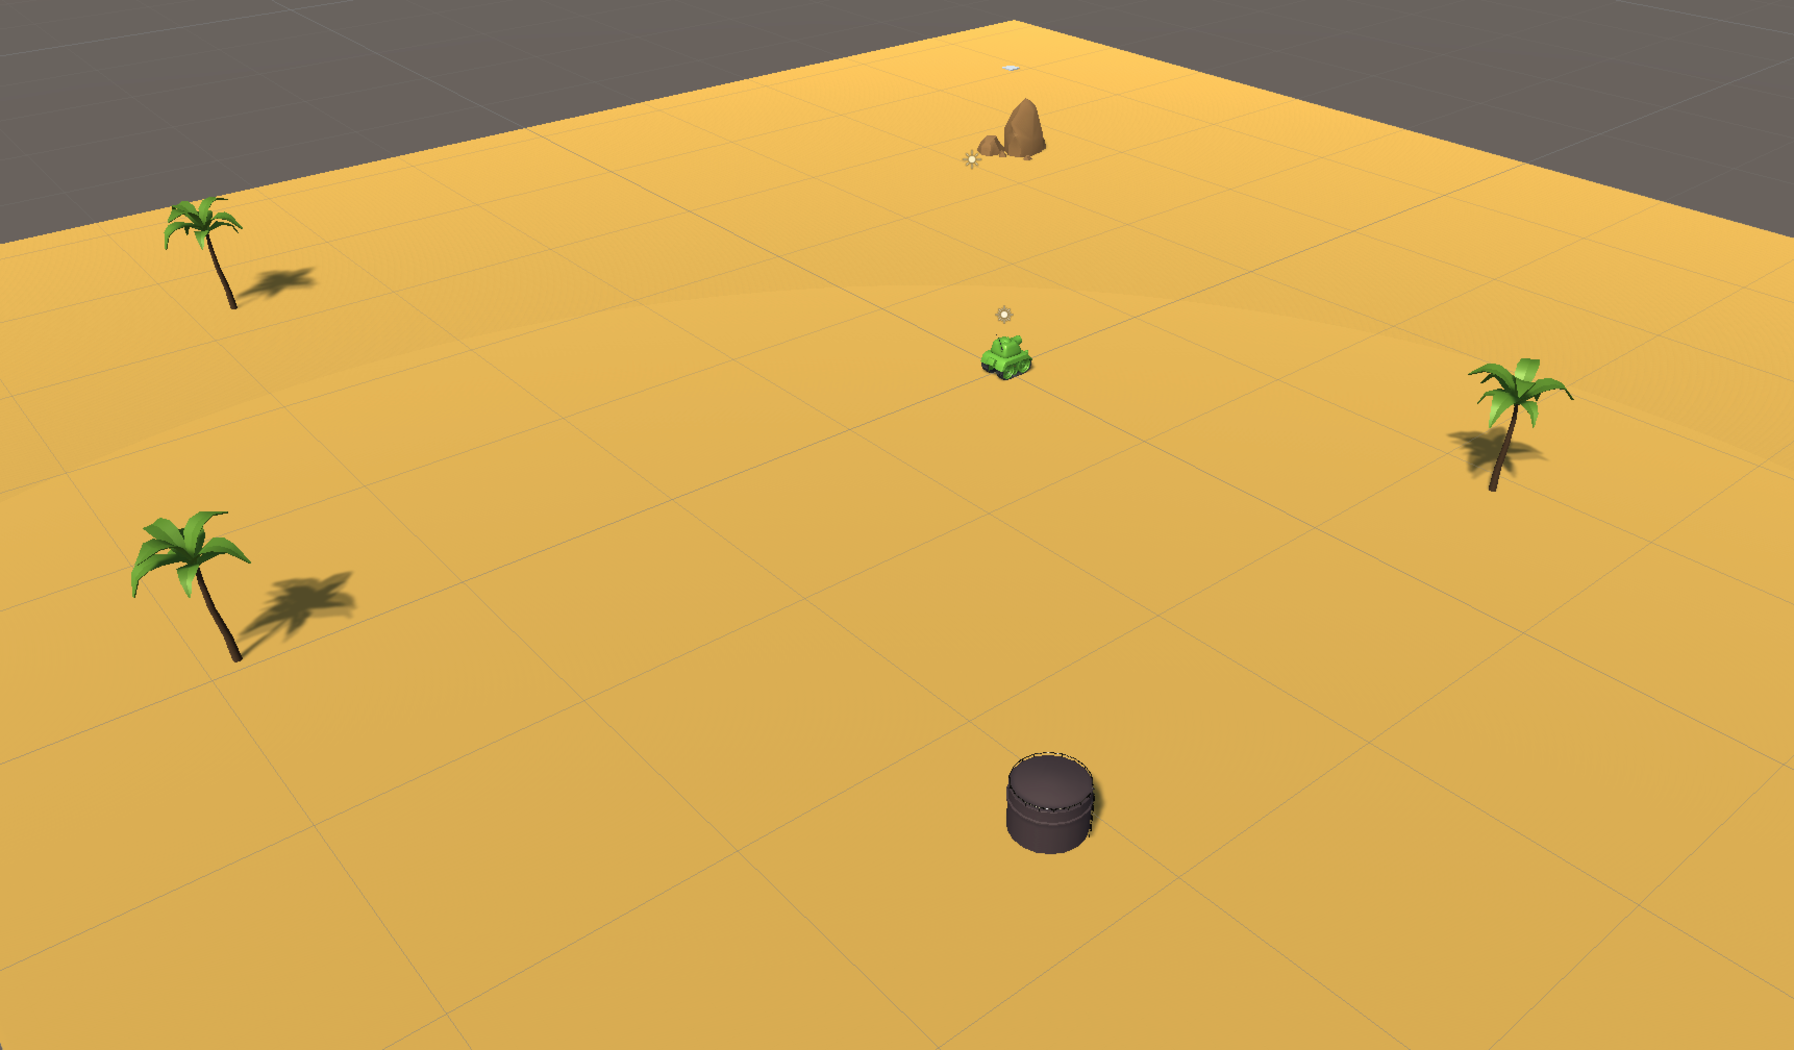
\includegraphics[height=0.5\columnwidth]{Chapter2/Map_2.pdf}\par
    \caption{Map of higher difficulty}
    \label{fig:map_2}
\end{figure}

\begin{figure*}[t]
\centering
\begin{multicols}{3}
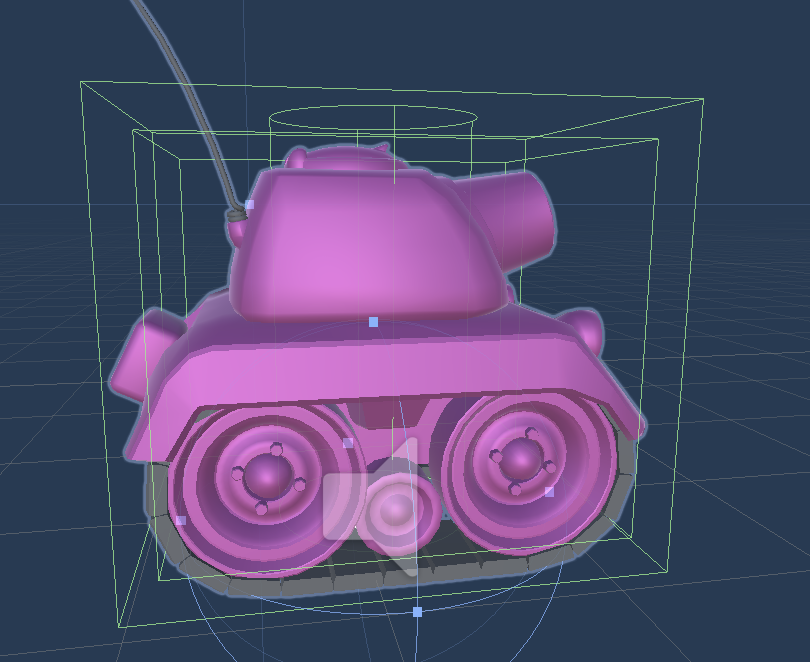
\includegraphics[width=0.99\columnwidth]{Chapter2/enemy_tank.png}\par
\caption{One of the Design of Enemy Tank}
\label{fig:enemy}


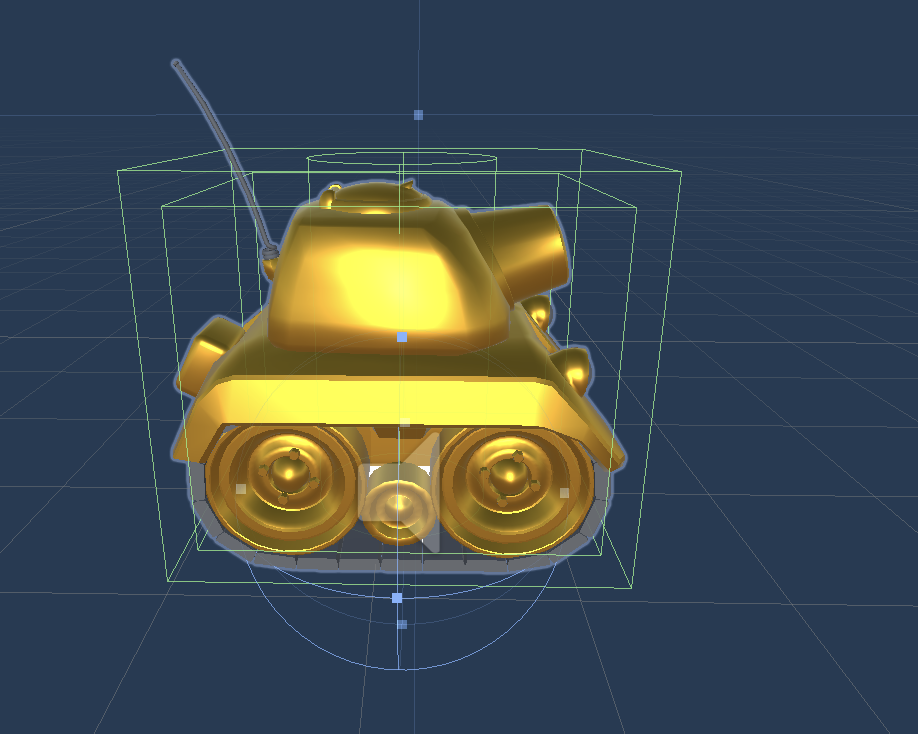
\includegraphics[width=0.99\columnwidth]{Chapter2/friendly_tank.png}\par
\caption{Design of Friendly Tank}
\label{fig:friendly}

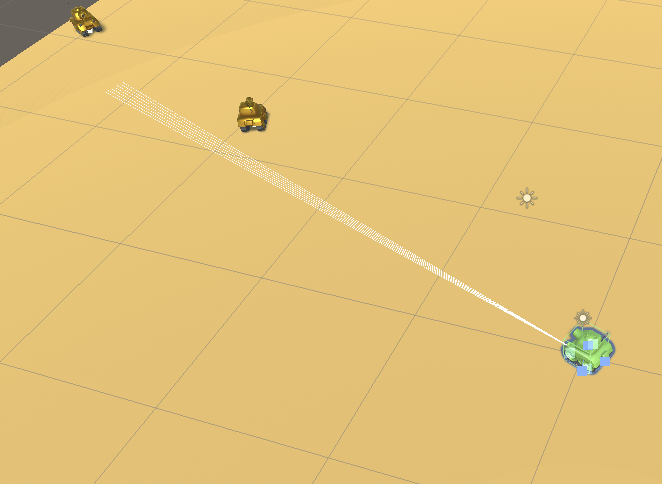
\includegraphics[width=0.99\columnwidth]{Chapter2/Raycast.png}\par
\caption{Agent Tank has limited range of Raycast to balance difficulty}
\label{fig:rays}
\end{multicols}
\end{figure*}

%=== END OF CHAPTER TWO ===
